\chapter{CƠ SỞ LÝ THUYẾT}
\subsection{Mạng nơ-ron đệ quy (RNN)}
\subsubsection{Kiến trúc mạng nơ-ron đệ quy RNN}
Con người không bắt đầu suy nghĩ của họ từ đầu tại tất cả các thời điểm. Cũng giống như việc đọc báo cáo đồ án này, chúng ta hiểu mỗi chữ ở đây dựa vào các chữ chúng ta đã hiểu trước đó chứ không phải đọc tới đâu ném hết đi tới đó, rồi bắt đầu suy nghĩ lại từ đầu tới chữ chúng ta đang đọc. Tức là tư duy đã có bộ nhớ để lưu lại những gì điễn ra trước đó.\par
Tuy nhiên các mô hình mạng nơ-ron truyền thống thì không thể làm được việc đó, đó có thể coi là một khuyết điểm chính của mạng nơ-ron truyền thống. Ví dụ, nếu chúng ta muốn phân loại các bối cảnh xảy ra ở tất cả các thời điểm trong một bộ phim, thì đúng là không thể hiểu được một tình huống trong phim mà lại phụ thuộc vào các tình huống trước đó nếu sử dụng các mạng nơ-ron truyền thống.\par
Mạng nơ-ron hồi quy (Recurrent Neural Network) sinh ra để giải quyết vấn đề đó. Mạng này chứa các vòng lặp bên trong cho phép thông tin có thể lưu lại được.\par
\begin{figure}[H]
    \centering
    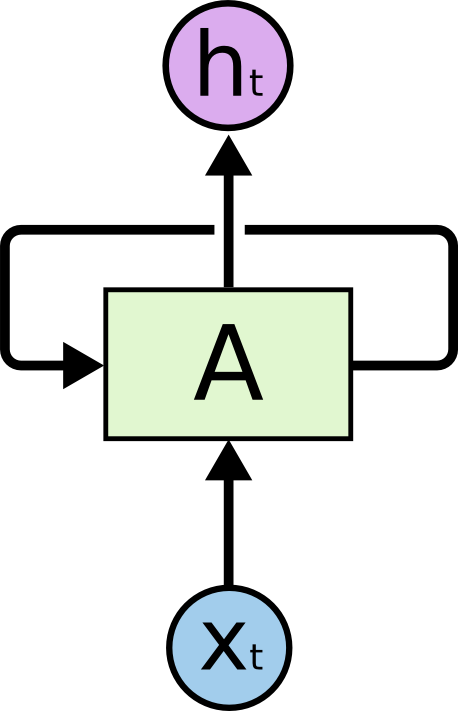
\includegraphics[scale=0.5]{figures/RNN-rolled.png}
    \caption{Recurrent Neural Networks have loops.}
\end{figure}
Hình vẽ trên mô tả một đoạn của mạng nơ-ron hồi quy $\mathcal{A}$ với đầu vào là $x_t$ và đầu ra là $h_t$. Một vòng lặp cho phép thông tin có thể được truyền từ bước này qua bước này qua bước khác của mạng nơ-ron.\par
Một mạng nơ-ron hồi quy có thể được coi là nhiều bản sao chép của cùng một mạng, trong đó mỗi đầu ra của mạng này là đầu vào của một mạng sao chép khác. Chuỗi lặp lại các mạng này chính là phân giải của mạng nơ-ron hồi quy, các vòng lặp khiến chúng tạo thành một chuỗi danh sách các mạng sao chép nhau. \par
\begin{figure}[H]
    \centering
    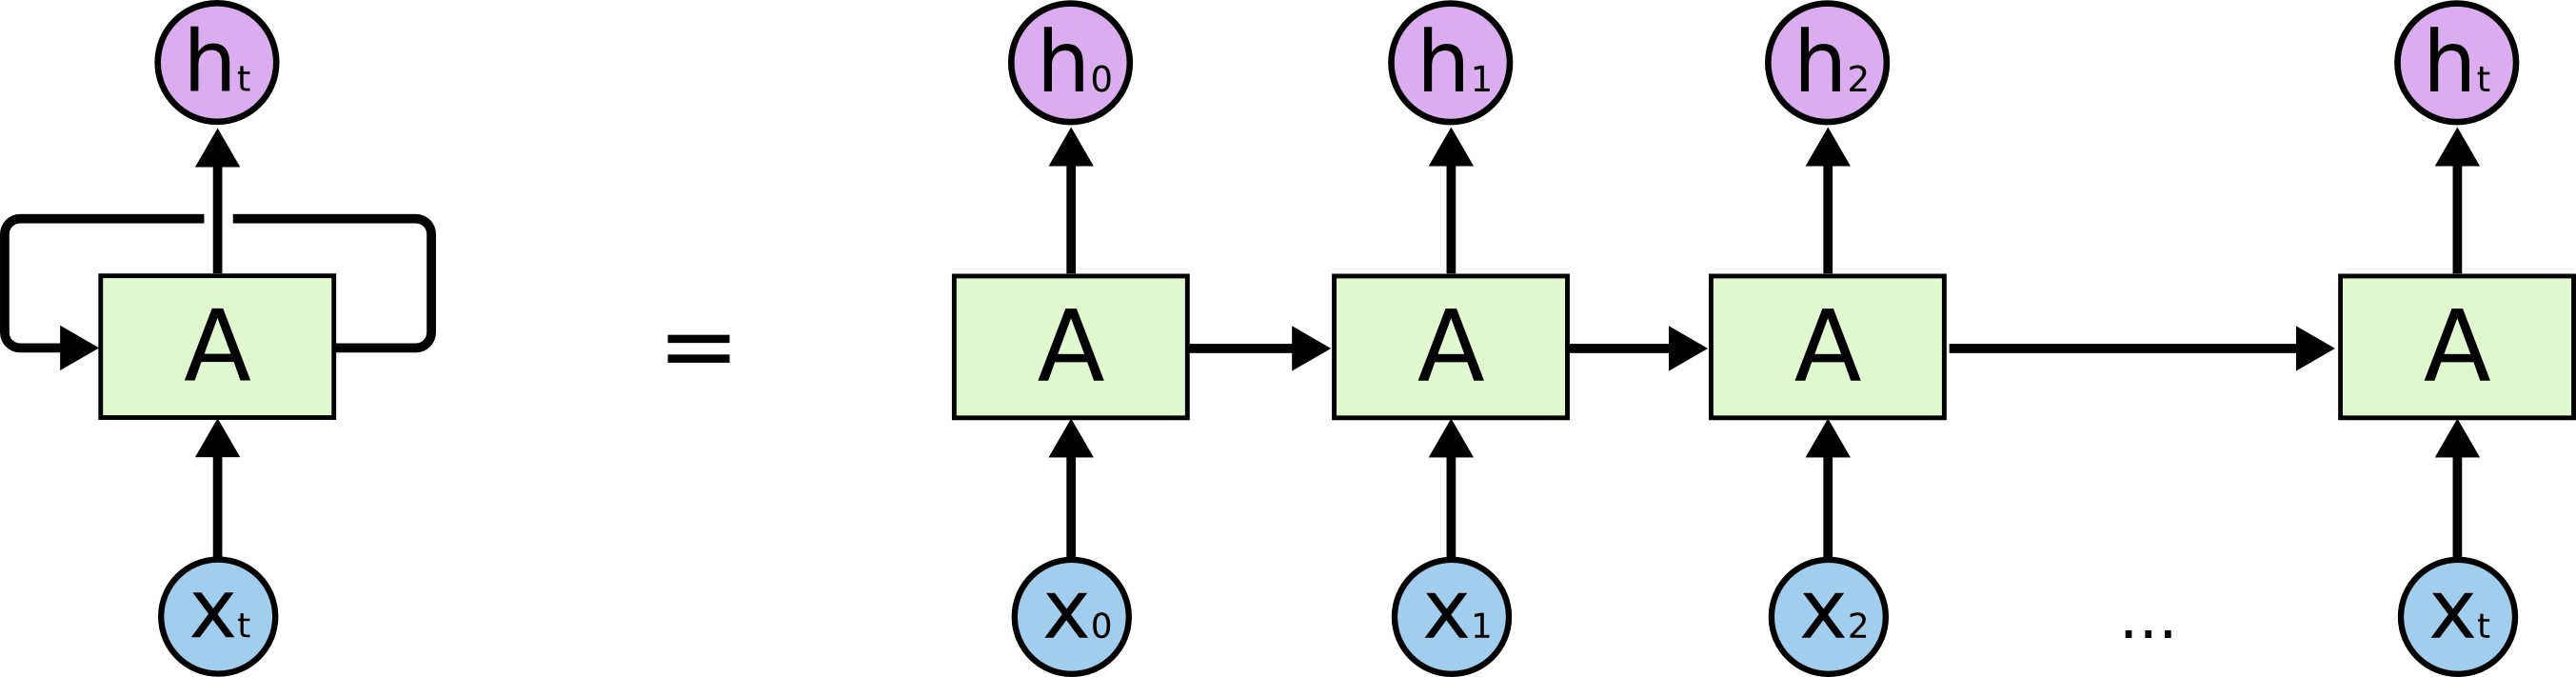
\includegraphics[width=0.75\textwidth]{figures/RNN-unrolled.png}
    \caption{An unrolled recurrent neural network.}
\end{figure}
Trong vài năm gần đây, việc ứng dụng RNN đã đưa ra được nhiều kết quả không thể tin nổi trong nhiều lĩnh vực: nhận dạng giọng nói, mô hình hóa ngôn ngữ, dịch máy, mô tả ảnh,… Danh sách vẫn còn đang được mở rộng tiếp.
\subsubsection{Vấn đề phụ thuộc xa}
Một điểm nổi bật của RNN chính là ý tưởng kết nối các thông tin phía trước để dự đoán cho hiện tại. Việc này tương tự như ta sử dụng các cảnh trước của bộ phim để hiểu được cảnh hiện thời. Nếu mà RNN có thể làm được việc đó thì chúng sẽ cực kì hữu dụng, tuy nhiên liệu chúng có thể làm được không?\par
Đôi lúc ta chỉ cần xem lại thông tin vừa có thôi là đủ để biết được tình huống hiện tại. Ví dụ, ta có câu: \textit{“các đám mây trên bầu trời”} thì ta chỉ cần đọc tới \textit{“các đám mây trên bầu”} là đủ biết được chữ tiếp theo là \textit{“trời”} rồi. Trong tình huống này, khoảng cách tới thông tin có được cần để dự đoán là nhỏ, nên RNN hoàn toàn có thể học được.\par
\begin{figure}[H]
    \centering
    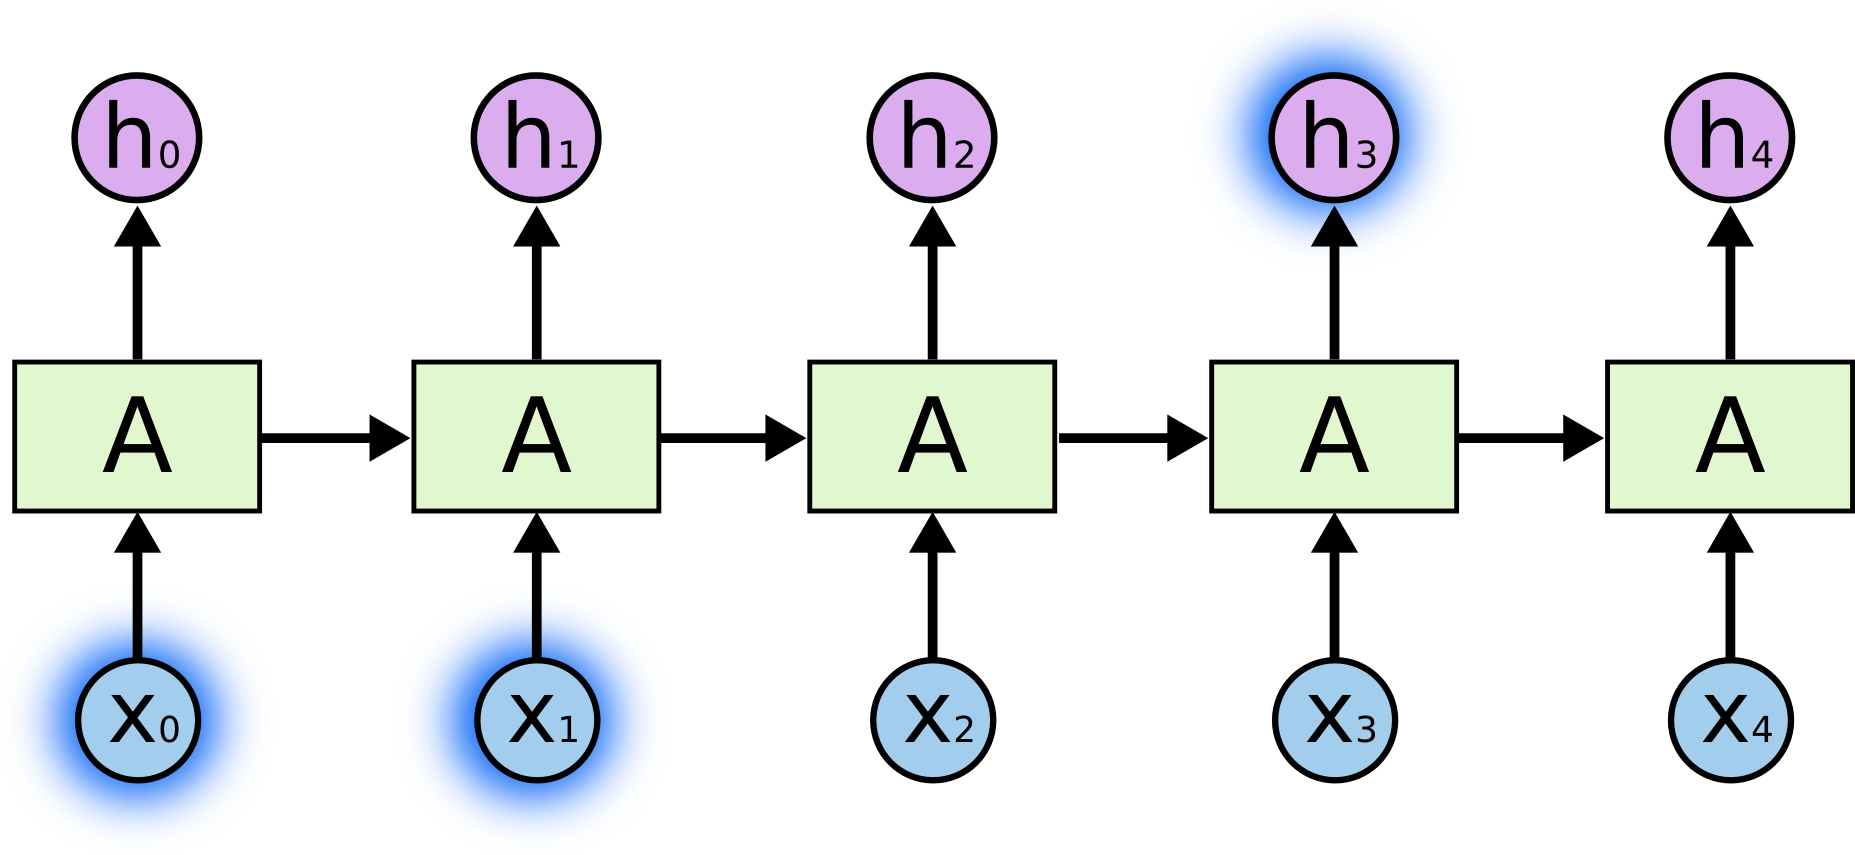
\includegraphics[width=0.7\textwidth]{figures/RNN-shorttermdepdencies.png}
    \caption{Mạng RNN phụ thuộc ngắn.}
\end{figure}
Nhưng trong nhiều tình huống ta buộc phải sử dụng nhiều ngữ cảnh hơn để suy luận. Ví dụ, dự đoán chữ cuối cùng trong đoạn: \textit{“I grew up in France… I speak fluent French.”}. Rõ ràng là các thông tin gần (\textit{”I speak fluent”}) chỉ có phép ta biết được đằng sau nó sẽ là tên của một ngôn ngữ nào đó, còn không thể nào biết được đó là tiếng gì. Muốn biết là tiếng gì, thì ta cần phải có thêm ngữ cảnh \textit{“I grew up in France”} nữa mới có thể suy luận được. Rõ ràng là khoảng cách thông tin lúc này có thể đã khá xa rồi.\par
Thật không may là với khoảng cách càng lớn dần thì RNN bắt đầu không thể nhớ và học được nữa.
\begin{figure}[H]
    \centering
    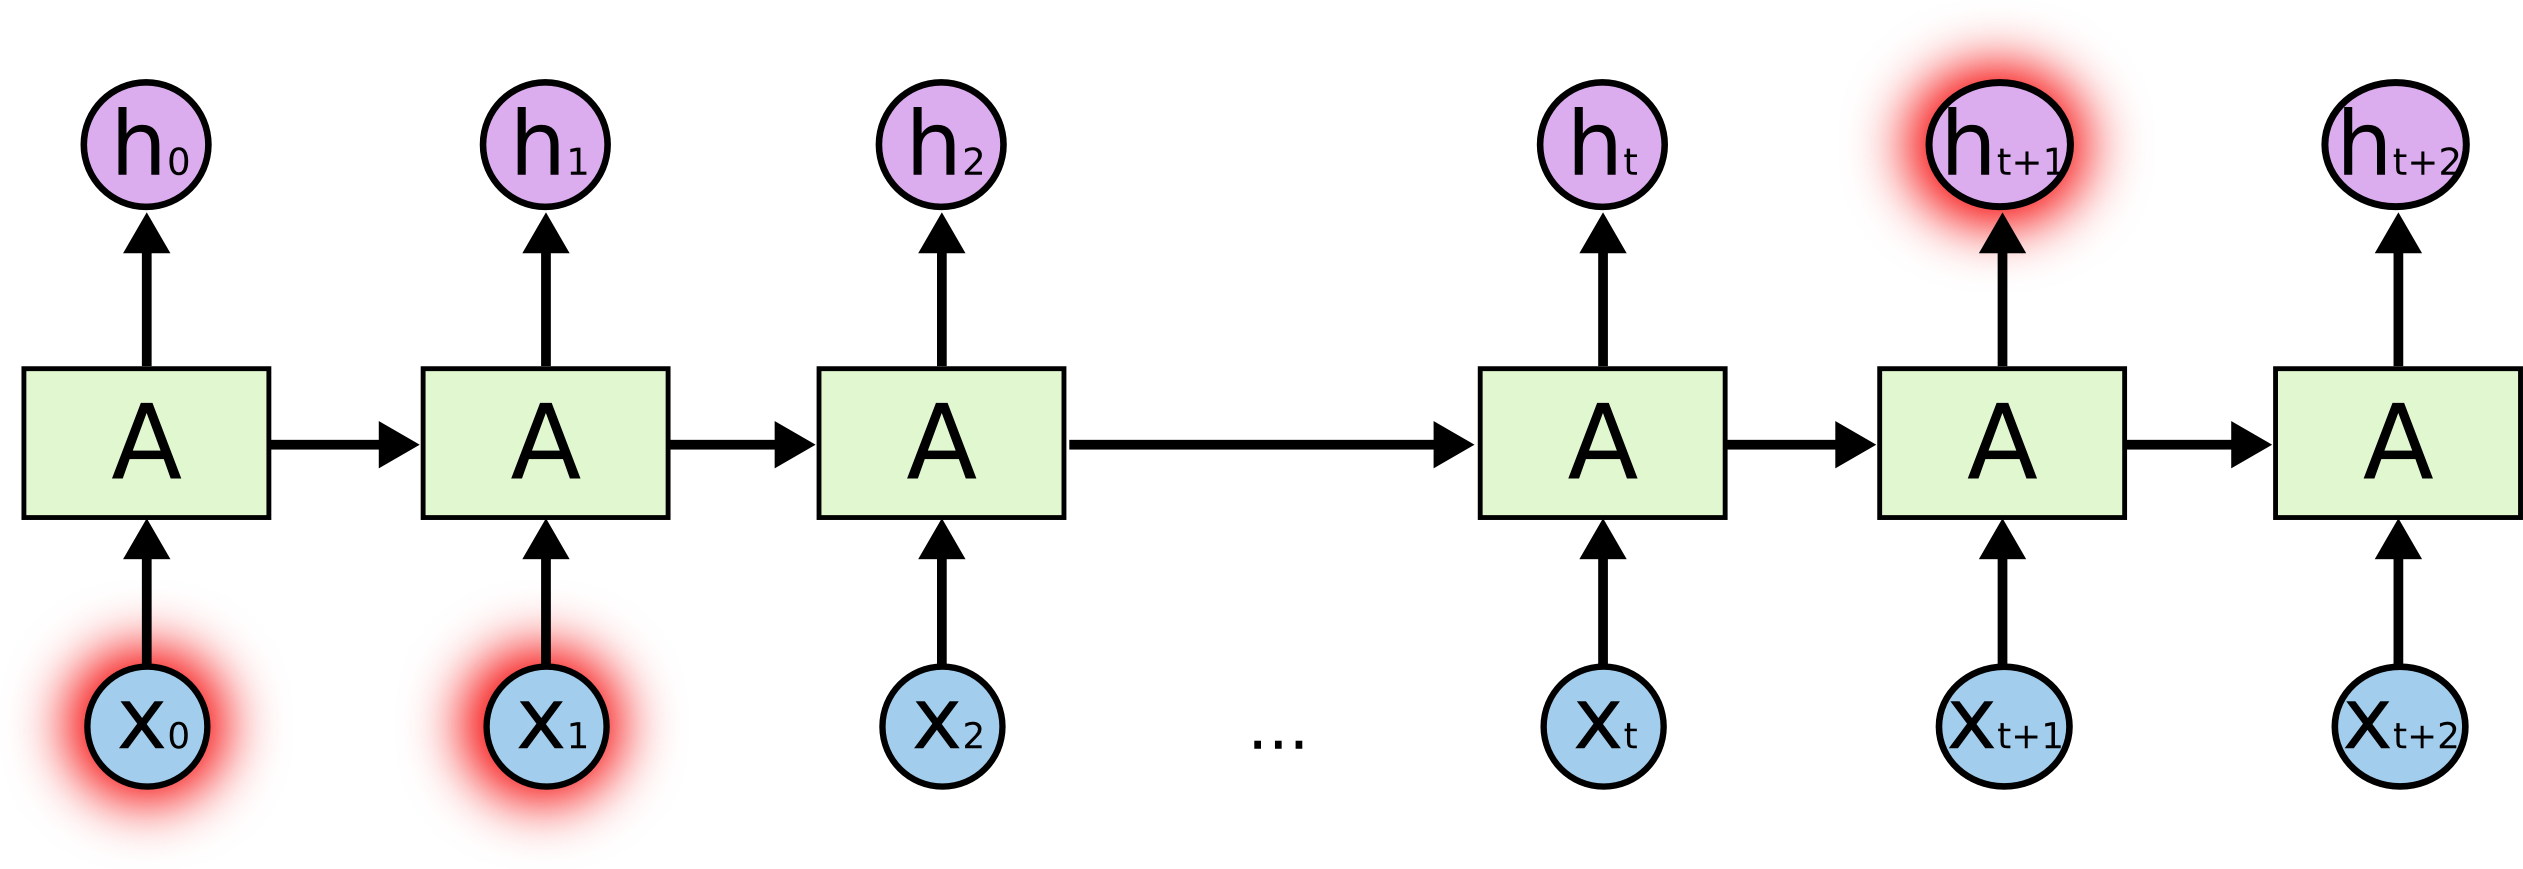
\includegraphics[width=0.75\textwidth]{figures/RNN-longtermdependencies.png}
    \caption{Mạng RNN phụ thuộc dài.}
\end{figure}
Về mặt lý thuyết, rõ ràng là RNN có khả năng xử lý các phụ thuộc xa (long-term dependencies). Chúng ta có thể xem xét và cài đặt các tham số sao cho khéo là có thể giải quyết được vấn đề này. Tuy nhiên, đáng tiếc trong thực tế RNN có vẻ không thể học được các tham số đó. Vấn đề này đã được khám phá khá sâu bởi \textbf{Hochreiter (1991)} và \textbf{Bengio, et al (1994)} trong các bài báo của mình, họ đã tìm được nhưng lý do căn bản để giải thích tại sao RNN không thể học được. \par
Tuy nhiên, LSTM không vấp phải vấn đề đó.
\section{LSTM}
\subsection{Mô hình Long Short Term Memory networks (LSTM)}
Mạng bộ nhớ dài-ngắn (Long Short Term Memory networks), thường được gọi là LSTM - là một phiên bản mở rộng của mạng thần kinh hồi quy (RNN) nhân tạo được sử dụng trong lĩnh vực học sâu. LSTM được giới thiệu bởi \textbf{Hochreiter \& Schmidhuber}  vào năm 1997.\par
LSTM được đưa ra để giải quyết các vấn đề về phụ thuộc xa (long-term dependency) trong mạng RNN do bị ảnh hưởng bởi vấn đề mất gradient. Việc nhớ thông tin trong suốt thời gian dài là đặc tính mặc định của LSTM, chứ không cần phải huấn luyện để có thể nhớ được. Tức là ngay nội tại của nó đã có thể ghi nhớ được mà không cần bất kì can thiệp nào.\par

Một đơn vị LSTM thông thường bao gồm:
\begin{itemize}
    \item \textbf{Tế bào (cell)}
    \item \textbf{Cổng quên (forget gate):} có nhiệm vụ loại bỏ những thông tin không cần thiết nhận được khỏi cell internal state.
    \item \textbf{Cổng vào (input gate):} có nhiệm vụ chọn lọc nhưng thông tin cần thiết nào được thêm vào cell internal state.
    \item \textbf{Cổng ra (output gate):} có nhiệm vụ xác định những thông tin nào từ cell internal state được sử dụng như đầu ra.
\end{itemize}
\begin{figure}[H]
    \centering
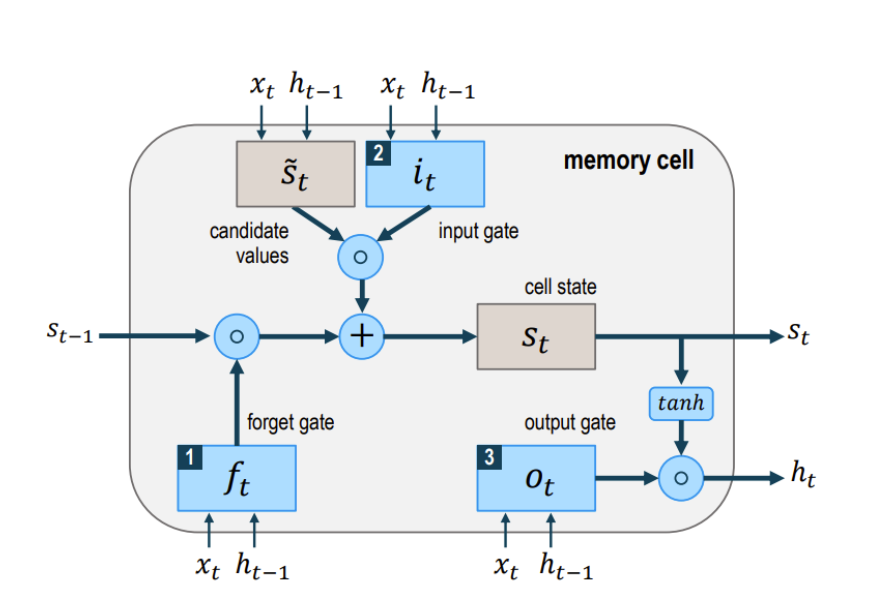
\includegraphics[width=0.7\textwidth]{figures/sodo.png}
    \caption{Sơ đồ biểu diễn kiến trúc bên trong của một tế bào LSTM}
\end{figure}

\subsubsection{Kiến trúc bên trong LSTM}
Bước đầu tiên của LSTM là quyết định xem thông tin nào cần bỏ đi từ trạng thái tế bào. Quyết định sẽ được  tầng sigmoid đưa ra hay còn gọi là tầng cổng quên (forget gate layer). Nó lấy đầu vào là $h_{t-1}$ và $x_t$  rồi đưa ra kết quả nằm trong khoảng $[0, 1]$ cho mỗi giá trị trong trạng thái tế bào $C_{t-1}$. Đẩu ra là $0$ chỉ rằng toàn bộ thông tin sẽ bị bỏ đi, còn $1$ thể hiện rằng nó giữ toàn bộ thông tin lại.\\

\begin{figure}[H]
    \centering
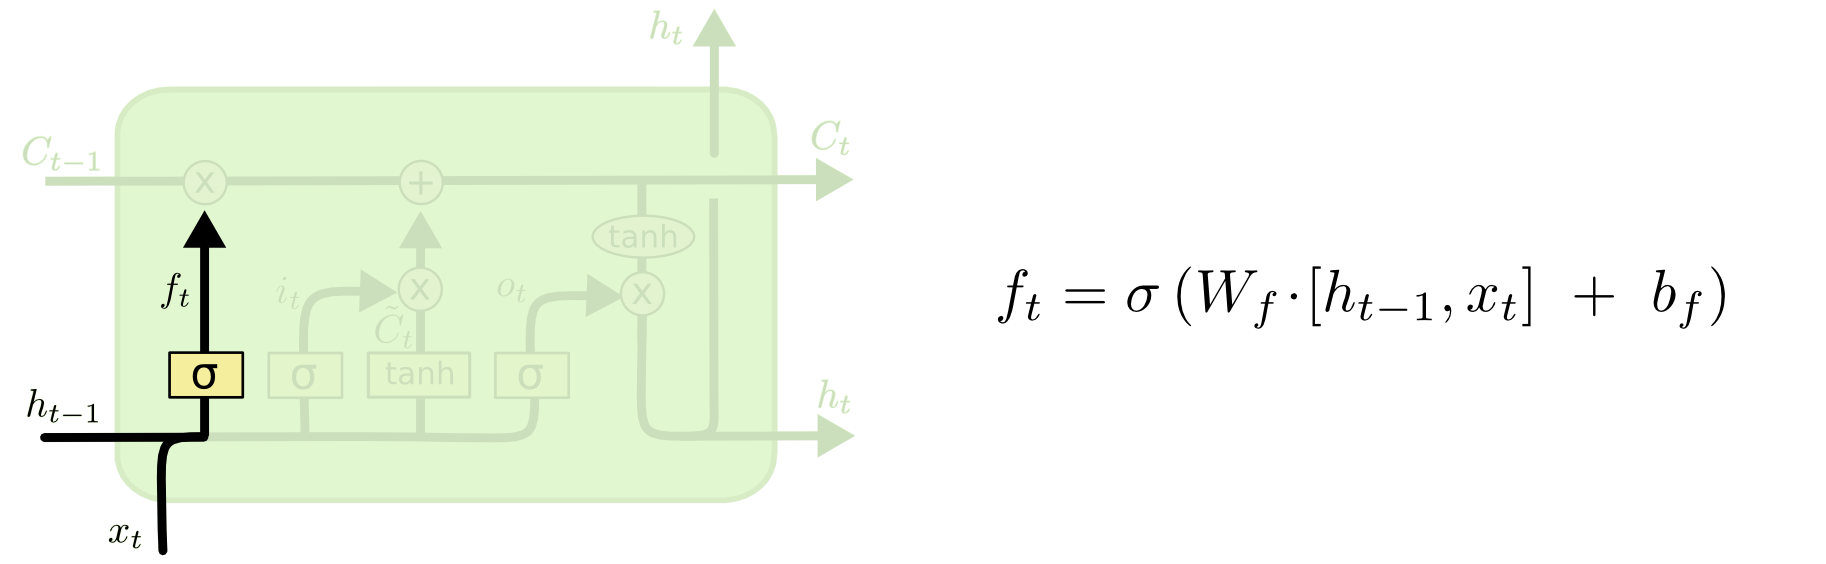
\includegraphics[width=0.9\textwidth]{figures/LSTM3-focus-f.png}
    \captionof{figure}[Tầng cổng quên]{Tầng cổng quên.}
\end{figure}
\par
Bước tiếp theo là quyết định xem thông tin mới nào ta sẽ lưu vào trạng thái tế bào. Việc này gồm 2 phần. Đầu tiên là sử dụng một tầng sigmoid - tầng cổng vào (input gate layer) để chọn giá trị cập nhật. Sau đó là tầng $tanh$ sẽ tạo ra một vector giá trị mới $\tilde{C_t}$ mục đích là thêm vào cho trạng thái. Trong bước kế tiếp ta sẽ kết hợp 2 giá trị trên với nhau nhằm mục đích tạo ra một cập nhật trang thái. \\
\begin{figure}[H]
    \centering
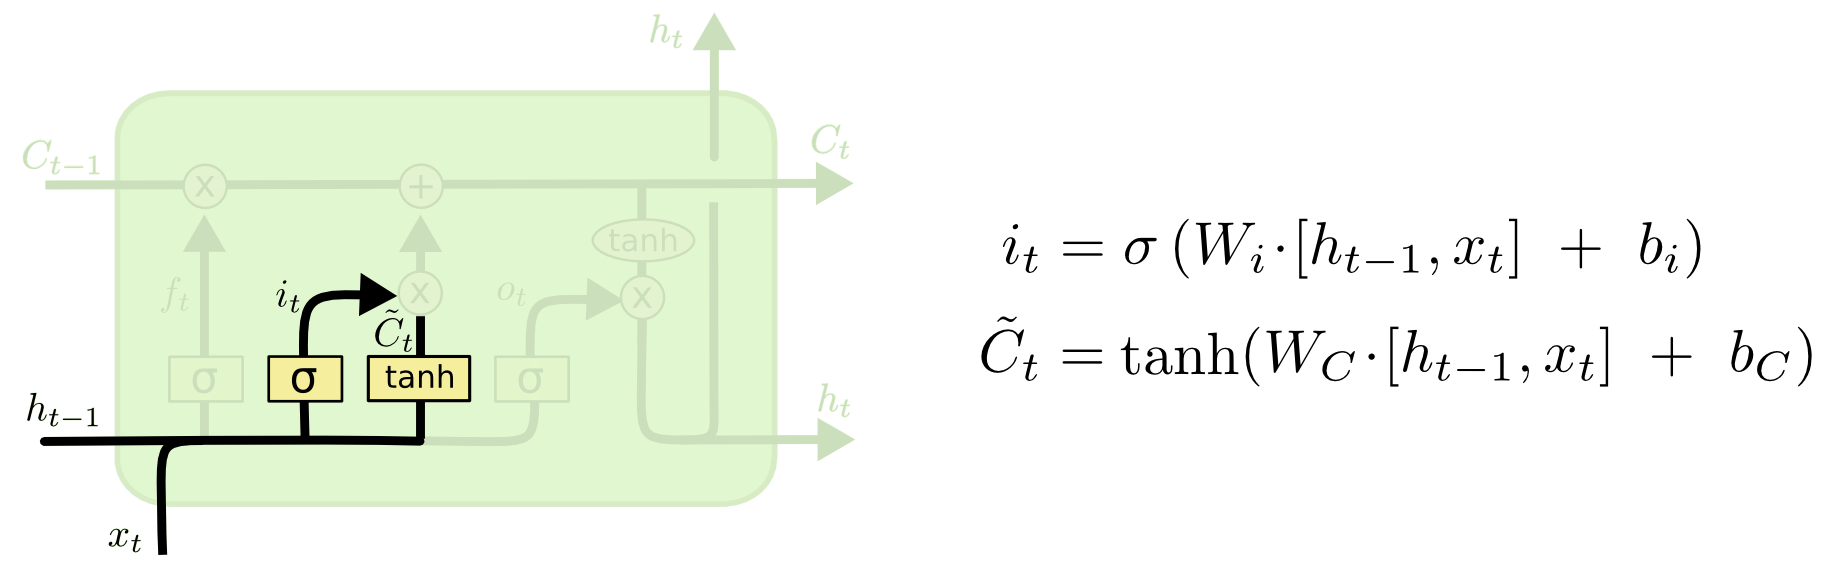
\includegraphics[width=0.9\textwidth]{figures/LSTM3-focus-i.png}
    \captionof{figure}[Tầng cổng vào]{Tầng cổng vào.}
\end{figure}

\par
Giờ là lúc cập nhập trạng thái tế bào cũ $C_{t-1}$  thành trạng thái mới $C_t$. Trong các bước trước đó đã quyết định các việc cần làm, nên bây giờ chỉ cần thực hiện.\\
Nhận trạng thái trước với $f_t$ để loại bỏ được những thông tin đã quyết định quên. Sau đó cộng thêm $i_t*\tilde{C_t}$. Trạng thái mơi thu được này phụ thuộc vào việc ta quyết định cập nhập mỗi giá trị trạng thái ra sao.\\
\begin{figure}[H]
\centering
	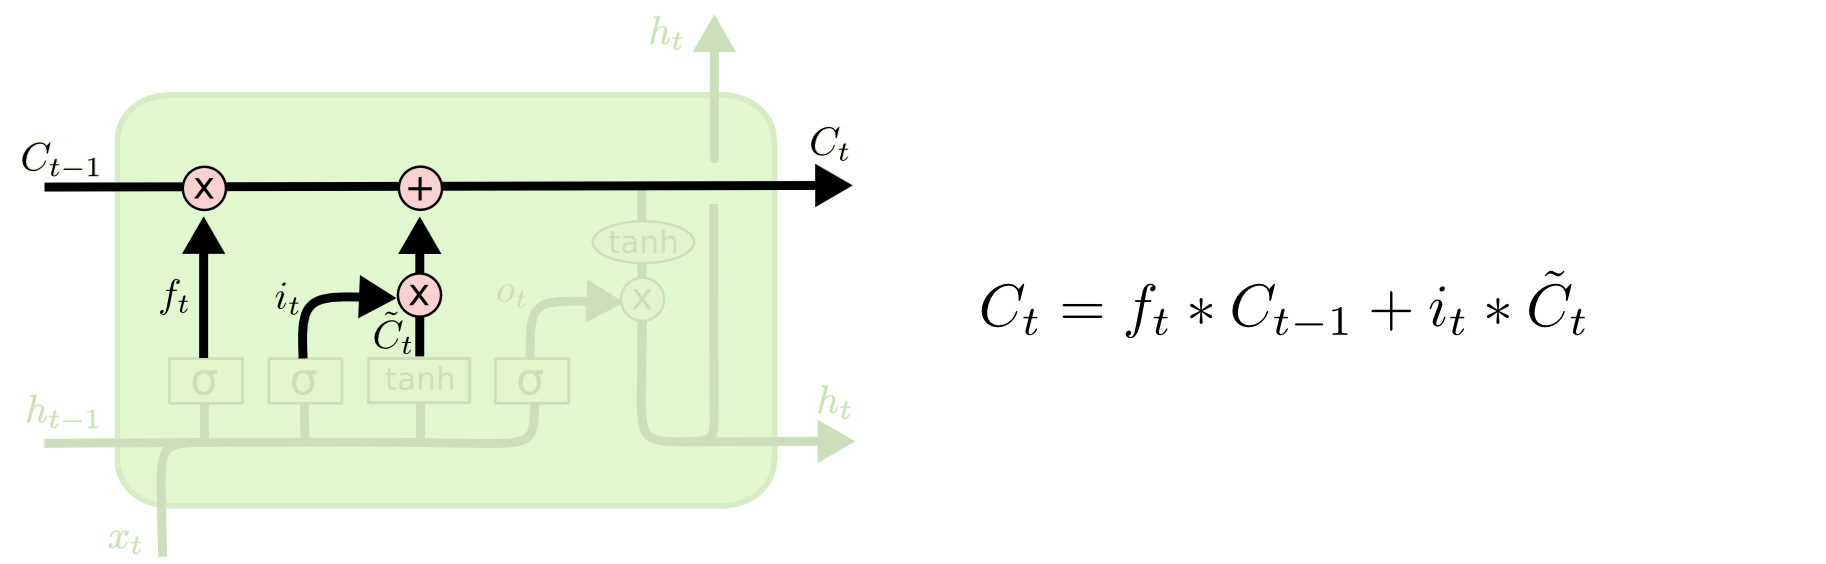
\includegraphics[width=0.9\textwidth]{figures/LSTM3-focus-C.png}
	\captionof{figure}[Cập nhật trạng thái tế bào]{Cập nhật trạng thái tế bào.}
\end{figure}

\par
Cuối cùng, ta cần xem xem đầu ra mong muốn là gì. Giá trị đầu ra sẽ dựa vào trạng thái tế bào và sẽ được tiếp tục sàng lọc. Trước tiên, ta chạy một tầng $sigmoid$ để chọn phần nào của trạng thái tế bào ta muốn xuất ra. Sau đó, ta đưa nó trạng thái tế bảo qua một hàm $tanh$ để co giá trị nó về khoảng $[-1, 1]$, và nhân nó với đầu ra của cổng sigmoid để được giá trị đầu ra ta mong muốn.
\begin{figure}[H]
\centering
	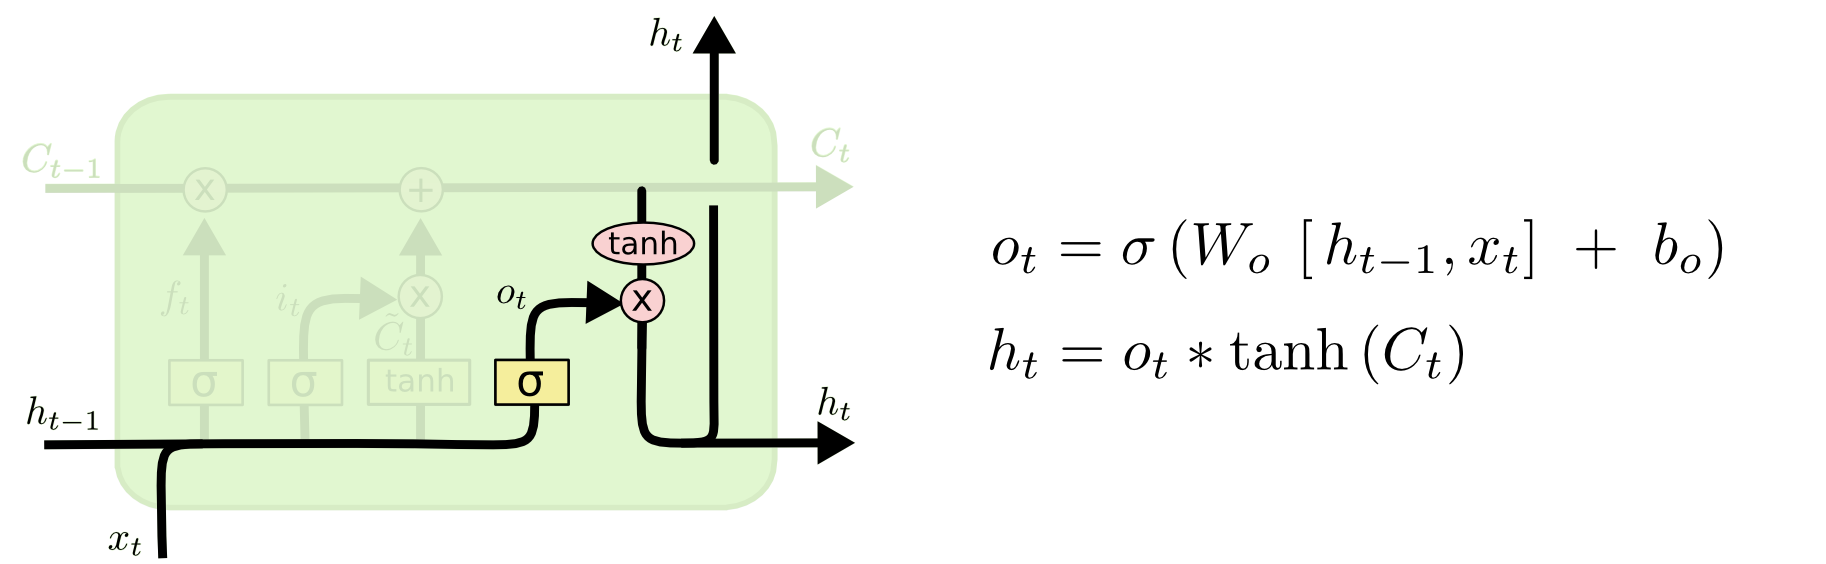
\includegraphics[width=0.9\textwidth]{figures/LSTM3-focus-o.png}
	\captionof{figure}[Cổng ra]{Cổng ra.}
\end{figure}

\section{VARMAX}
\subsection{Giới thiệu mô hình VARMAX}
Mô hình tự hồi quy trung bình trượt véc tơ với các biến hồi quy ngoại sinh (VARMAX). Đường tự hồi quy trung bình trượt véc tơ với các biến hồi quy ngoại sinh (VARMAX) là một phần mở rộng của mô hình VARMA cũng bao gồm mô hình hóa các biến ngoại sinh. Nó là phiên bản đa biến của phương pháp ARMAX.

Các biến ngoại sinh còn được gọi là đồng biến và có thể được coi là các chuỗi đầu vào song song có các quan sát ở các bước đồng thời với chuỗi ban đầu. (Các) chuỗi chính được gọi là dữ liệu nội sinh để đối chiếu nó với (các) chuỗi ngoại sinh. Các quan sát đối với các biến ngoại sinh được đưa trực tiếp vào mô hình tại mỗi bước thời gian và không được mô hình hóa theo cách giống như chuỗi nội sinh chính (ví dụ như quy trình AR, MA, v.v.).

Mô hình VARMAX là một mô hình phù hợp cho chuỗi thời gian đa biến. Nó thêm thành phần trung bình cộng vào mô hình VAR và có thể cho phép các biến ngoại sinh. Bởi vậy, mô hình VARMAX gồm các thành phần:
\begin{itemize}
    \item \textbf{VAR (Vector Autoregression):} thành phần tự hồi quy bao gồm tập hợp các độ trễ của biến hiện tại.
    \item \textbf{MA (Moving Average):} được hiểu là quá trình thay đổi hoặc dịch chuyển giá trị trung bình của một chuỗi theo thời gian.
    \item \textbf{X (Exogenous variable):} sử dụng các biến ngoại sinh.
\end{itemize}
Mô hình này có thể phù hợp với các quy trình phức tạp hơn nhiều mô hình chuỗi thời gian khác. Tuy nhiên, nó cũng có nhược điểm: thời gian train tương đối dài so với các mô hình đơn giản hơn và cần một lượng dữ liệu tương đối lớn để ước tính chính xác.

\subsection{Mô hình VARMAX(p,q)}
Mô hình toán học của VARMAX được định nghĩa như sau:
Công thức tổng quát cho mô hình VARMAX:
        $$X_t = \delta_t - \Sigma_{i=0}^p\phi_i X_{t-i} + \varepsilon_t + \Sigma_{i=1}^q \theta_i \varepsilon_{t-i}$$
        hay $\phi(B)X_t = \delta_t + \theta(B)\varepsilon_t$ \\
        tại $\phi(B) = I_k - \Sigma^p_{i=1}\phi_i B^i$, $\theta(B)=I_k-\Sigma^q_{i=1}\theta_i B^i$ \\
        và $\delta_t$ có thể là một hằng số xác định (biến ngoại sinh).


Các thành phần của VARMAX:
\begin{itemize}
		\item Auto regression: Kí hiệu là AR. Đây là thành phần tự hồi quy bao	gồm tập hợp các độ trễ của biến hiện tại. Mô hình AR có thể được biểu diễn như sau:\par
		\begin{equation}
		    y_{t}=c+\phi_{1}y_{t-1}+\epsilon_{t}
		\end{equation}
		Trong đó: $y_t$ là giá trị tại thời gian t, c là hằng số, $\Phi_1$ là hệ số còn $\epsilon_t$ là nhiễu trắng với $\epsilon_t \sim N(0, \sigma^2)$.
		
		Độ trễ bậc p chính là giá trị lùi về quá khứ p bước thời gian của chuỗi. Độ trễ dài hoặc ngắn trong quá trình AR phụ thuộc vào tham số trễ p. Mô hình AR(p) của chuỗi $y_t$ được biểu diễn như sau:\par
		\begin{equation}
		    y_{t}=c+\phi_{1}y_{t-1}+\phi_{2}y_{t-2}...+\phi_{p}y_{t-p}+\epsilon_{t}
		\end{equation}
		    hay\par
		\begin{equation}
		    y_{t}=c+\sum_{i=1}^{p}\phi_{i}y_{t-i}
		\end{equation}
		
		    Trong đó $\Phi_i$ là hệ số tương ứng của mỗi giá trị $y{_t-i}$.\par
		\item 	Moving average: Quá trình trung bình trượt được hiểu là quá trình dịch chuyển hoặc thay đổi giá trị trung bình của chuỗi theo thời gian. Do chuỗi của chúng ta được giả định là dừng nên quá trình thay đổi trung bình dường như là 1 chuỗi nhiễu trắng. Quá trình moving average sẽ tìm mối liên hệ về mặt tuyến tính giữa các phần tử ngẫu nhiên $\epsilon_t$ chuỗi này là 1 chuỗi nhiễu trắng có các tính chất:\par
		\begin{align}
		    E(\epsilon_{t})=0\label{hang1}\\
		    \sigma(\epsilon_{t})=\alpha	\label{hang2}\\
		     \rho(\epsilon_{t},\epsilon_{t-s)}=0, \forall  t\geq s\label{hang3}
		\end{align}
		Vế \eqref{hang1} có nghĩa rằng kì vọng của chuỗi dừng bằng 0 để đảm bảo chuỗi dừng không có sự thay đổi về trung bình theo thời gian. Vế \eqref{hang2} là phương sai của chuỗi không đổi. Do kì vọng và phương sai không đỏi nên chúng tagọi phân phối của nhiễu trắng là phân phối xác định và được kí hiệu $\epsilon_t \sim \mathcal{WN}(\ {0},\,\sigma^{2})$. Nhiễu trắng là một thành phần ngẫu nhiên thể hiện cho yếu tố không thể dự báo của model và không có tính quy luật. Quá trình trung bình trượt được biểu diễn theo nhiễu trắng như sau:\par
		\begin{equation}
		    MA(q)=\mu+\sum_{i=1}^{q}\theta_{i}\epsilon_{t-i}
		\end{equation}
	\end{itemize}

 \subsection{Cách xác định hệ số p, q}
 \subsubsection{Cách xác định hệ số p của AR}
     Để kiểm tra hệ số q của mô hình AR ta kiểm tra biểu đồ tự tương quan 1 phần (PACF). \par
     Tự tương quan một phần có thể được hình dung như mối tương quan giữa chuỗi và độ trễ của nó, sau khi loại trừ các đóng góp từ độ trễ trung gian. Vì vậy, PACF truyền tải mối tương quan thuần túy giữa độ trễ và chuỗi. Bằng cách đó, ta sẽ biết liệu độ trễ đó có cần thiết trong điều kiện AR hay không.\par
     Bất kỳ sự tự tương quan nào trong một chuỗi dừng đều có thể được điều chỉnh bằng cách thêm đủ các thuật ngữ AR. Vì vậy, ban đầu ta coi thứ tự của số hạng AR bằng với càng nhiều độ trễ vượt qua giới hạn ý nghĩa trong biểu đồ PACF.\par
\begin{figure}[H]
    \centering
    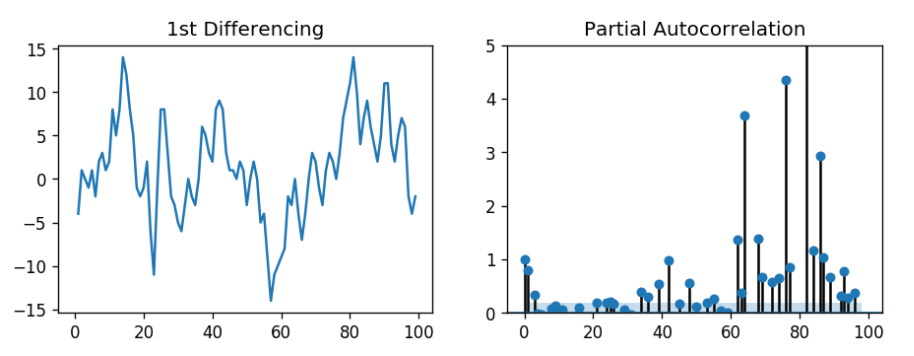
\includegraphics[scale=0.8]{figures/PACF.png}
    \caption{Ví dụ cách xác định p}
\end{figure}     
     Có thể quan sát thấy rằng độ trễ PACF bằng 1 là khá đáng kể vì nằm trên đường ý nghĩa (vùng màu xanh lam). Vì vậy ta chọn p bằng 1.
\subsubsection{Cách xác định hệ số q của MA}
     Cũng giống như cách xem xét biểu đồ PACF cho hệ số của AR, chúng ta có thể xem biểu đồ ACF để biết hệ số của MA.\par
\begin{figure}[H]
    \centering
    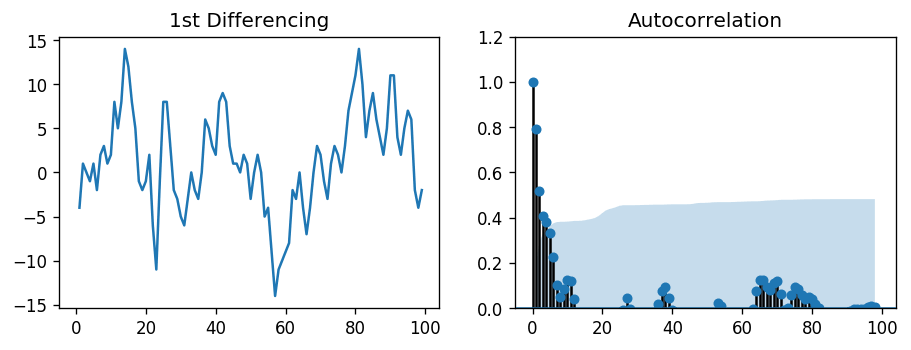
\includegraphics[scale=0.45]{figures/ACF.png}
    \caption{Ví dụ cách xác định q}
\end{figure}
     Biểu đồ ACF cho ta biết cần phải thực hiện quá trình MA bao nhiêu lần để loại bỏ sự tự tương quan trong chuỗi thời gian dừng. Ở đây ta thấy nhiều là nằm trên đường ý nghĩa, ta có thể chọn giá trị q là 1 hoặc 2.
\subsection{Ước lượng tham số mô hình sử dụng thuật toán đổi mới}
     Giả sử ta có một chuỗi ARMA(p,q) dừng với các quan sát $X_{t}, t=1,2,...,N$. Mô hình \text{ARMA(p,q)} đưa ra bởi $X_t$:\par
     \begin{equation}
         \phi(B)X_{t}=\theta(B)Z_{t}
     \end{equation}\par
     Với $\phi(B)$ và $\theta(B)$ là các đa thức bậc p và q\par
     \begin{equation}
         \phi(B)=1-\phi_{1}B-...-\phi_{p}B^{p}
     \end{equation}\par
     và\par
     \begin{equation}\label{ARMA(1)}
         \theta(B)=1+\theta_{1}B+...\theta_{q}B^{q}
     \end{equation}\par
     Với B là toán tử lùi xác định bởi ($B^{j}X_{t}=X_{t-j}, B^{j}Z_{t}=Z_{t-j}, j=0,\pm1,...$), $Z_{t}$ là chuỗi nhiễu trắng với kỳ vọng bằng 0 và phương sai là $\sigma^{2}$.\par
     \begin{equation}\label{ARMA(2)}
         X_{t}-\phi_{1}X_{t-1}-...-\phi_{p}X_{t-p}=Z_{t}+\theta_{1}Z_{t-1}+...\theta_{q}Z_{t-q}
     \end{equation}\par
     Khi p=0 thì biểu thức \eqref{ARMA(2)} là một chuỗi MA(q) còn nếu q=0 thì biểu thức \eqref{ARMA(2)} là một chuỗi AR(p). Brockwell và Davis (1987) đã đưa ra một thuật toán để ước tính các tham số AR và MA cho một mô hình ARMA (p, q). Theo đó, với hàm tự tương phương sai đã biết(ACVF) $\gamma(.)$ thì các ước lượng đổi mới $\theta_{1,1},\theta_{2,2},\theta_{2,1},\theta_{3,3},\theta_{3,2},...$ có thể có được theo các biểu thức:\par
     \begin{align}
         V_{0}=\gamma(0)\label{ARMA(3)}\\
         \theta_{m,m-k}=V_{k}^{-1}[\gamma(m-k)-\sum_{j=0}^{k-1}\theta_{m,m-j}]\label{ARMA(4)}\\
         V_{m}=\gamma(0)-\sum_{j=0}^{m-1}\theta_{m,m-j}V_{j}\label{ARMA(5)}
     \end{align}\par
     Nếu quá trình được cho bởi phương trình \eqref{ARMA(1)} là khả nghịch, thì nó có thể được biểu diễn dưới dạng:\par
     \begin{equation}
         X_t=\sum_{j=0}^{\infty}\psi_{j} W_{t-j}\label{ARMA(6)}
     \end{equation}\par
     Biểu thức \eqref{ARMA(1)} và \eqref{ARMA(6)} có thể được biểu diễn:\par
     \begin{align}
         \psi_{0}=1\label{ARMA(7)}\\
         \psi_{j}=\theta_{j}+\sum_{i=1}^{min(j,p)}\theta_{i}\psi_{j-1}, j=1,2,...\label{ARMA(8)}
     \end{align}\par
     Theo quy ước ta có $\theta_{j}=0$ với j > q và $\phi_{i}=0$ với i > p của chuỗi ARMA(p,q). Brockwell và Davis (1987) còn chứng minh thêm rằng $\psi_{j}\longrightarrow\theta_{m,j}$. Do đó biểu thức\eqref{ARMA(8)} được viết dưới dạng:\par
     \begin{equation}
         \theta_{m,j}=\theta_{j}+\sum_{i=1}^{min(j,p)}\phi_{i}\theta_{m,j-1},j=1,2,...p+q\label{ARMA(9)}
     \end{equation}\par
     Với j=q+1, q+2,...q+p trong biểu thức \eqref{ARMA(9)} một hệ p phương trình có thể được tạo ra và chúng có dạng:\par
     \begin{equation}\label{ARMA(10)}
         \begin{bmatrix}
               \theta_{m,q+1}\\
               \theta_{m,q+2}\\
               \vdots\\
               \theta_{m,q+p}
         \end{bmatrix}
         =\
         \begin{bmatrix}
               \theta_{m,q}&\theta_{m,q-1}&\cdots&\theta_{m,q+1-p}\\
               \theta_{m,q+1}&\theta_{m,q}&\cdots&\theta_{m,q+2-p}\\
               \vdots&\vdots&\cdots&\vdots\\
               \theta_{m,q+p-1}&\theta_{m,q+p-2}&\cdots&\theta_{m,q}
         \end{bmatrix}
         \begin{bmatrix}
               \phi_1\\
               \phi_2\\
               \vdots\\
               \phi_p
         \end{bmatrix}
     \end{equation}\par
      Các giá trị của ($\phi_{1},\phi_{2},...\phi_{p}$) có thể được xác định bởi biểu thức\eqref{ARMA(10)}. Từ biểu thức \eqref{ARMA(9)}, $\theta_{j}$ có thể được xác định bởi phương trình:\par
      \begin{equation}\label{ARMA(11)}
          \theta_{j}=\theta_{m,j}-\sum_{i=1}^{min(j,p)}\phi_{i}\theta_{m,j-i},j=1,2,...q
      \end{equation}\par
      Các kỹ thuật ở trên có thể được sử dụng để xác định tham số của AR và MA $\phi_{1},\phi_{2},...\phi_{p},\theta_{1},\theta_{2},...,\theta_{q}$ trong mô hình ARMA.